% !TEX TS-program = pdflatexmk
\documentclass[11pt]{article}
\usepackage[margin=.8in]{geometry}
\usepackage{amsmath,amssymb,amsthm, latexsym, mathrsfs, pdfsync, multicol,
fancybox, fancyhdr,
graphicx, enumerate,
subfig, tikz, pgfplots,array}

%\singlespacing
\def\RR{{\mathbb R}}
\def\NN{{\mathbb N}}
\def\ZZ{{\mathbb Z}}
\def\QQ{{\mathbb Q}}
\def\CC{{\mathbb C}}
\def\bc{\begin{center}}
\def\ec{\end{center}}
\def\be{\begin{enumerate}}
\def\ee{\end{enumerate}}
\def\bi{\begin{itemize}}
\def\ei{\end{itemize}}
\def\t{\times}
\newcommand{\ol}[1]{\overline{#1}}
\newcommand{\oimp}[1]{\overset{#1}{\Longleftrightarrow}}
\newcommand{\bv}[1]{\ensuremath{ \mathbf{\vec{#1}}} }
\renewcommand{\d}{\displaystyle}
\newcommand{\blank}[1]{\rule{#1}{0.75pt}}

\usetikzlibrary{calc}

\lhead{\sc{Math 316 Hist. of Math.}}
\chead{\large \sc Midterm I} 
\rhead{\sc Spring 2023}
\cfoot{}
\pagestyle{fancy}
%
\begin{document}
\thispagestyle{fancy}

\vspace{1in}
\begin{tabular}{ll}
\textbf{Student Name:}\hspace{1.5in}& \textbf{Proctor Name}\\
&\\
start time \hspace{1.5in} & end time\\
\end{tabular}

\vspace{1in}

{
\renewcommand{\baselinestretch}{1.8}
\setlength{\tabcolsep}{.2in}
\normalsize
\begin{center}
\begin{tabular}{|c|c|c|c|}
\hline
&Problem&Total Points&\parbox{.8in}{\hfil Score\hfil}\\
\hline
Part I&&25&\\
\hline
Part II &&&\\
\hline
&1&8&\\
\hline
&2&8&\\
\hline
&3&11&\\
\hline
&4&8&\\
\hline
&5&10&\\
\hline
&6&30&\\
\hline
\hline
Total&100&&\\
\hline
\end{tabular}

\end{center}
}

\vspace{1in} 

Guidelines
\begin{itemize}
\item You have 1 hour to take the exam.
\item The exam will be given in two parts.
\item Part I is written without any aids: no notes, no book, no phone. You should spend no more than 15 minutes on Part I. 
\item Turn your completed Part I to the proctor and you will be given Part II. You cannot return to Part I once you have turned it in.
\item For Part II, you may use a calculator and two pages of notes (i.e. two sheets of paper).
\end{itemize}

\newpage
\vspace*{-0.3in}

\bc Part I \ec

This part is written without notes or aids of any kind. It is worth 25 points out of 100 total points. \\

Below is a list of eight mathematicians or mathematical documents. Give a detailed description of \textbf{five of the eight}.  A complete description will include approximate dates, location, and mathematical significance. \\

Once you have completed Part I and turn it in, you will be given Part II. You cannot return to Part I once it has been turned in.\\

\be
\item Rhind Papyrus
\vfill
\item Moscow Papyrus
\vfill
\item Plimpton 322
\vfill
\newpage
\item Thales of Miletus
\vfill
\item Pythagoras of Samos
\vfill
\item Euclid
\vfill
\item Theon of Smyrna
\vfill
\item Eudoxus of Cnidos
\vfill
\ee
\newpage 

\bc Part II \ec

For this part, you may use a calculator and up to two pages of notes. This part is worth 75 points out of 100 total points.

\be
%%%add-subtract like a mayan
\item (8 points) Demonstrate \emph{using Mayan symbols} how ancient Mayans must have performed subtraction below.

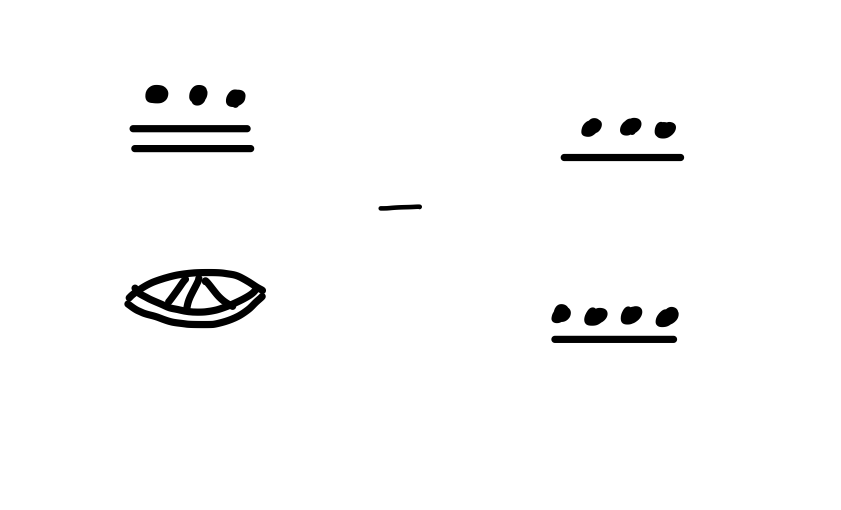
\includegraphics[scale=0.5]{mayan.jpeg}
\vfill

%%%%% multiply - divide like an Egyptian
\item (8 points) Use the ancient Egyptian method to divide 47 by 18.
\vfill
\newpage
%%%%% Fractions base 60 and division like Babylonian
\item (11 points)
	\be
	\item Write the base 60 number $(3,45)$ in base 10.
	\vfill
	\item Explain how $(3,45)$ could be viewed by ancient Babylonians as the reciprocal of 16. Your answer should include a computation.
	\vfill
	\ee

%%% Figurative numbers
\item (8 points) Give a proof-by-picture proof that the sum of two consecutive triangular numbers is a square number. 
\vfill
\newpage
%%%Method of False position
\item (10 points) Solve the problem below using the method of false position. 
\begin{quote} A quantity, its half, and its fifth added together becomes two. What is the quantity? \end{quote}
\vfill


%%%%%
\item (30 points) Short Answer
	\be
	\item Give an example of a numerical system of representation that is \emph{additive} and another example that is \emph{positional} and explain the difference.
	\vfill
	\item Greek mathematicians starting using an \emph{alphabetic} or \emph{ciphered} numeral system by the 5th century b.c. Explain what an alphabetic numeral system is, its advantages and disadvantages.
	\vfill
\newpage
	\item Describe two impressive accomplishments of ancient Egyptian mathematicians.
	\vfill
	\item Compare the Babylonian approach to quadratic equations with the modern approach.
	\vfill
	\item Explain what \textbf{ancient Greeks mathematicians} meant by the statement ``the diagonal of a square and its side are incommensurable." 
	\vfill 
	\ee
\ee
\end{document}
%%%%%%%%%%%%%%%%%%%%%%%%%%
%%%%%%%END
%%%%%%%%%%%%%%%%%%%%%%%%%%


 